\cleardoublepage
\chapter{Introduction}
\label{ch:introduction}
\begin{fullwidth}
  \newthought{In the 6th century B.C.} Pythagoras discovered that
  dividing a resonating string into simple mathematical ratios
  produced harmonious musical intervals, while arbitrary ratios
  produced dissonance.  His observation is probably the first of the
  many explicit parallels between math and music that have been
  identified after his time. Today, we describe musical pitches, as
  integers within a given tuning system. We describe the tuning system
  with a mathematical formula that relates frequency to pitch. Musical
  time, rhythm and meter are commonly described numerically. Musical
  Transposition and inversion mirror mathematical functions, and
  borrow their names directly from mathematics.
\end{fullwidth}

As computers, amplifiers, and electronics become our primary tools for
creating manipulating, and performing music, mathematics and music
also become more interconnected. Nearly every modern musical
recording, broadcast, and stream is the summation of many digital
recordings that have been individually discretized, sampled
mathematically encoded, decoded, and digitally processed numerous
times before ever reaching our ears.\cite{Case2007} We might be
tempted to describe music today as applied mathematics, but doing so
betrays a fundamental quality of music: Musicality does not correspond
to mathematical elegance or precision. A musician will diverge from a
musical score to accomplish a particular artistic objective. A
vocalist does not abruptly change a pitch, but gently and carefully
lands on a pitch. A jazz musician might play slightly behind the
beat. A classical performer knows how to hold a fermata just long
enough. These intentional human artifacts are characterized more by a
feeling than by a formula.

The computer's inability to understand feeling has led to new genres
of music like EDM\sidenote[][-25mm]{EDM (Electronic Dance Music) often
  features formulaic and repetitive grooves locked to a temporal grid,
  and incorporates aggressive use of digital pitch correction
  exaggerating a robotic quality.}, Black MIDI\sidenote[][-3mm]{Black
  MIDI is a musical genre that uses low fidelity audio samplers with a
  large number of MIDI notes over a short time. A single 3 minute
  Black MIDI track is likely to have over 100,000 MIDI notes. The name
  refers to the solid black appearance of the piano score.}, and
Demoscene\sidenote{Demoscene music celebrates digital synthesis of
  compositionally complex electronic music and audio visualizations,
  using low level software interfaces, and including the design and
  programming of the music synthesizers as part of the composition.},
but these styles of music feature (rather than fix) the inhuman nature
of computers. If we want to integrate a computer into the performance
or production of truly expressive music, we must capture perceived
feelings formulaically, and program the computer to reproduce
them. This thesis describes three different but related projects that
confront this challenge from contrasting perspectives: \refmod,
\polytempic, and \thesis.

\section{\refmod}
\label{sec:refmod-intro}
\newthought {Music and space} are intimately connected. This project
explores how we can compose music using acoustic reflections in
architectural space as a medium. \refmod is a software tool that lets
us design and experiment with abstract acoustic lenses or ``sound
mirrors'' in 2 dimensions. It is directly inspired by the music and
architecture of Iannis Xenakis, a 20th century composer, music
theorist, architect and engineer. His collected works provide a guide
and perspective to all the projects in this thesis.

\section{\polytempic}
\label{sec:polytempic-intro}

\newthought{Music and Time} are inseparable. All music flows through
time, and depends on temporal constructs - the most common being meter
and tempo. Accelerating or decelerating tempo are common in many
styles of music, as are polyrhythms.  Music with multiple simultaneous
tempos or \textit{polytempic music} is less common, but still many
examples can be found. Few examples of music with simultaneous tempi
that shift relative to each other exist, and it is difficult for
musicians to accurately perform multiple tempi in parallel. Software
is an obvious choice for composing complex and challenging rhythms,
but modern compositional software makes this difficult. \polytempic
describes a strategy for composing music with multiple simultaneous
tempos that accelerate and decelerate relative to each other. In
\autoref{ch:polytempic} we derive an equation for smoothly ramping
tempi to converge and diverge as musical events within a score. We
show how this equation can be as a stochastic process to compose
previously inaccessible sonorities. 

\marginnote[10mm]{Unless noted otherwise, ``compression'' is used in this
  thesis to describe dynamic range compression, as opposed to data
  compression.}
\section{\thesis}
\label{sec:hypercompression-intro}
\newthought{We usually think of compression} in terms of
\emph{reduction}: We use data compression to reduce bit-rates and file
sizes, audio compression to reduce dynamic range. Record labels use
dynamic range compression as a weapon in the \emph{loudness
  war}\sidenote{``Loudness War'' is the popular name given to the
  trend of increasing percieved loudness in music recordings.
  Beginning in the 1990s, record labels have attempted to make their
  music louder than the competition, at the expense of audio
  fidelity}\cite{Deruty2014a}, resulting in some of today's music
recordings utilizing no more dynamic range than a 1909 Edison
cylinder.\cite{Katz2007}. A deeper study of dynamic range compression
reveals more subtle and artistic applications. A skilled audio
engineer applies compression to audio with the intention to improve
intelligibility, augment articulation, smooth a performance, shape
transients, extract ambience, de-ess vocals, balance multiple signals,
or even add distortion.\cite{Case2007} At its best, the compressor is
a tool for temporal shaping, rather than a tool for dynamic reduction.

\thesis expands the traditional model of a dynamic range compressor to
include spatial shaping. While unconventional, spatial
processing is a very natural fit for the compression paradigm. We can
think of sound as a medium that exists in time just as easily as we
can think of sound as something that exists in
space.\sidenote{Converting measurement of sound from the cycles per
  second (in the temporal domain) to wavelength (in the spatial
  domain) is common objective in acoustics and audio engineering
  practices. See \textit{The Sound Reinforcement Handbook} by G. Davis
  for examples.} The mathematics and implementation of the
Hypercompressor are described in detail in \autoref{ch:hypercompressor}.

\paragraph{Performance}
\thesis was used in the live performance of \textit{De
  L'Exp\'{e}rience}, a new musical work by composer Tod Machover for
Narrator, Organ, and Electronics. During the premier at the Maison
symphonique de Montr\'{e}al in Canada, \thesis was used to blend the
electronics with the organ and the acoustic space. In
\autoref{ch:hypercompressor} we also describe how Hypercompression fit
into this performance.

\section{Background}
\label{sec:background}
These projects build on the work and ideas of Iannis Xenakis, a 20th
century composer, architect, and engineer. Xenakis spent his youth
reading about astronomy, archeology, ancient literature, and
mathematics.\cite[]{Hoffmann2015} He studied music and engineering at
the Polytechnic Institute in Athens, Greece. By 1948, Xenakis had
graduated form the University, and moved to France where he began to
work for the french architect, Le Corbusier. The job put his
engineering skills to use, but he wanted to continute studying and
writing music.  While searching for a music mentor, he approached
Oliver Messiaen\sidenote{Messiaen was a prolific french composer
  known for rhythmic complexity. He was also regarded as an fantastic music
  teacher, and his students include Karlheinz Stockhausen, Pierre
  Boulez, and Quincy Jones.}, and asked if he should study harmony or
counterpoint. Messiaen later described his conversation with Xenakis:
\begin{quotation}``I think one should study harmony and
  counterpoint. But this was a man so much out of the ordinary that I
  said: No, you are almost 30, you have the good fortune of being
  Greek, of being an architect and having studied special
  mathematics. Take advantage of these things. Do them in your
  music.''\cite{Service2013}
\end{quotation}
Ultimately, Messiaen was rejecting Xenakis as a student, but we can
see how Xenakis did draw from disparate skills in his composition. The
score for his 1945 composition \textit{Metastasis}
(figure~\ref{fig:metastasis}), resembles an architectural blueprint as
much as it does a musical score.

\begin{figure*}[h]
  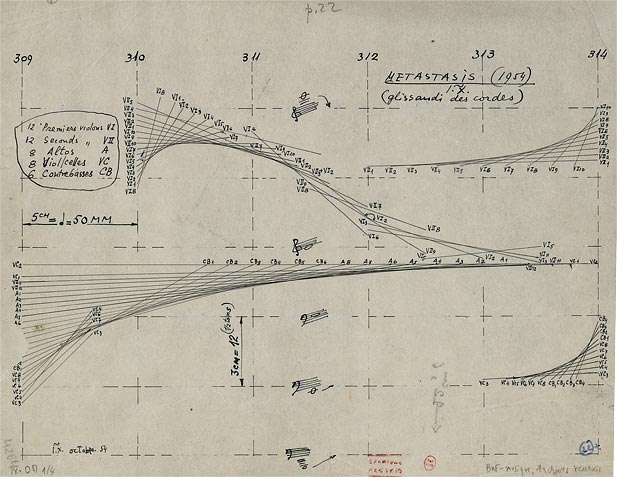
\includegraphics[width=\linewidth]{XenakisMetastasis.jpg}
  \caption{Excerpt from Iannis Xenakis' composition,
    \textit{Metastasis} (1954), measures 309-314. This score in this
    image was then transcribed to sheet music for the orchestral
    performance.}
  \label{fig:metastasis}
\end{figure*}

\subsection{The Philips Pavilion}
\label{sec:philips-pavilion-1}
\begin{figure}[h]
  \includegraphics[width=\linewidth]{PhilipsPavilion-TechnicalReview-01.pdf}
  \caption{The Philips Pavilion at the 1958 Brussels World Fair as
    shown in Volume 20 of the \textit{Philips Technical Review}, 1959}
  \label{fig:philips-pavilion-photo}
\end{figure}
In 1956, Le Corbusier was approached by Louis Kalff (Artistic Director
for the Philips corporation) and asked to build a pavilion for the
1958 World's Fair in Brussels. The pavilion was to showcase the sound
and lighting potential of Philips' technologies. Le Corbusier
immediately accepted, saying:
\begin{quotation}
  ``I will not make a pavilion for you but an Electronic Poem and a
  vessel containing the poem; light, color image, rhythm and sound
  joined together in an organic synthesis.''\cite{Lopez2011} 
\end{quotation}
The final product lived up to Le Corbusier's initial description. It
included:\cite{Lombardo2009}
\begin{enumerate}
\item A concrete pavilion, designed by architect and composer Iannis
  Xenakis
\item \textit{Interlude Sonoire} (later renamed \textit{Concret PH}), a
  tape music composition by Iannis Xenakis, approximately 2 minutes
  long, played between performances, while one audience left and
  pavillion, and the next audience another arrived.
\item A three channel, 8 minute tape music composition, by French-born
  composer Edgard Var\`{e}se
\item A system for spatialized audio across at least 350 loudspeakers
  distributed throughout the pavilion
\item An assortment of colored lighting effects, designed by Le Corbusier in
  collaboration with Philips art director Louis Kalff
\item Video consisting mostly of black and white still images,
  projected on two walls inside the pavilion
\item A system for synchronizing playback of audio and video,
  with the light effects and audio spatialization throughout the
  experience
\end{enumerate} 

\paragraph{The Role of Iannis Xenakis} During the initial design stage,
Le Corbusier determined that the shape of the pavilion building should
resemble a stomach, with the audience entering through one entrance,
and exiting through another. He completed initial sketches of the
pavilion layout, and then delegated the remainder of the design to
Xenakis.\cite{Clarke2012}

The architectural evolution of the pavilion from Le Corbusier's early
designs (figure~\ref{fig:le-corbusier-sketch}) through Xenakis'
iterations (figure~\ref{fig:xenakis-draw}), illustrates the impact
that Xenakis had on the project. An article in the \textit{Philips
  Technical Review}\cite{philips1958} gives a wonderfully detailed
account of Xenakis' process:
\begin{enumerate}
\item Xenakis was aware that parallel walls, or concave spherical
  walls would negatively impact audio perceptibility due to repeated
  or localized acoustic reflections.
\item To accommodate musical purpose of the space he decided to
  explore surfaces with varying curvature...
\item 
  \begin{marginfigure}
    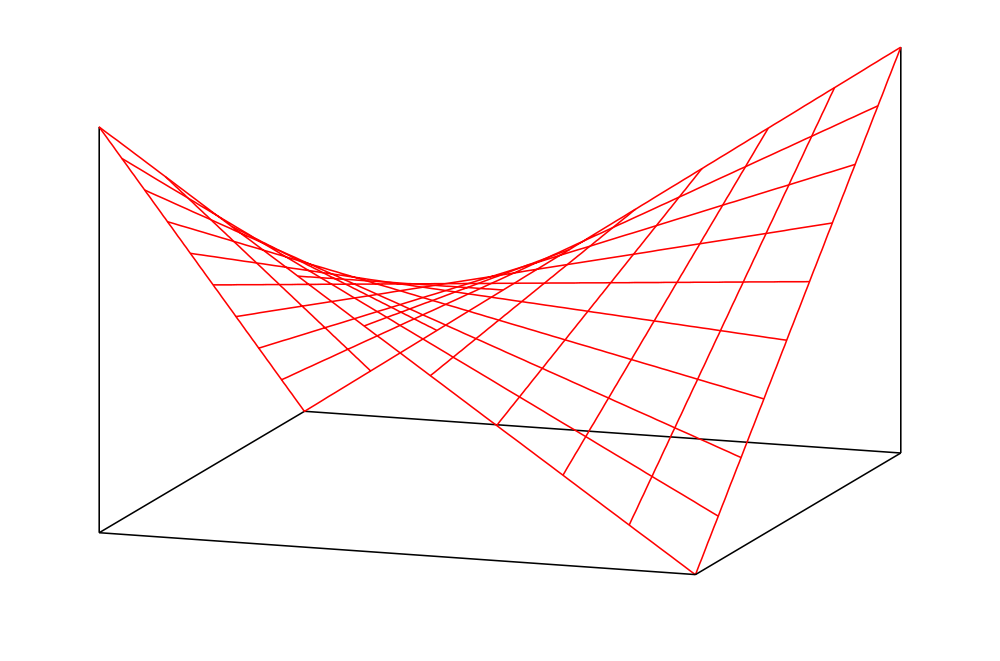
\includegraphics{hyperbolic-paraboloid}
    \caption{A ruled surface. For a surface to be considered ``ruled''
      every point on the surface must be on a straight line, and that
      line must lie on the surface. In Xenakis' time, ruled surfaces
      were useful in architecture, because they simplified the
      construction of curved surfaces by using straight beams.}
    \label{fig:ruled-surface}
  \end{marginfigure}...leading him to consider ruled surfaces such as
  the conoid and hyperbolic paraboloid. 
\end{enumerate}
We see Xenakis utilizing the drafting skills that he learned at the
Polytechnic Institute and continued to develop while working with Le
Corbusier. He also understood the mathematical formation of the ruled
surfaces that make up the structure. These surfaces even look familiar
from the Metastasis score (figure~\ref{fig:metastasis}). In his book
1963 book, \textit{Formalized Music}, Xenakis explicitly states that
the philips pavilion was inspired by his work on
\textit{Metastasis}.

\begin{figure*}[]
  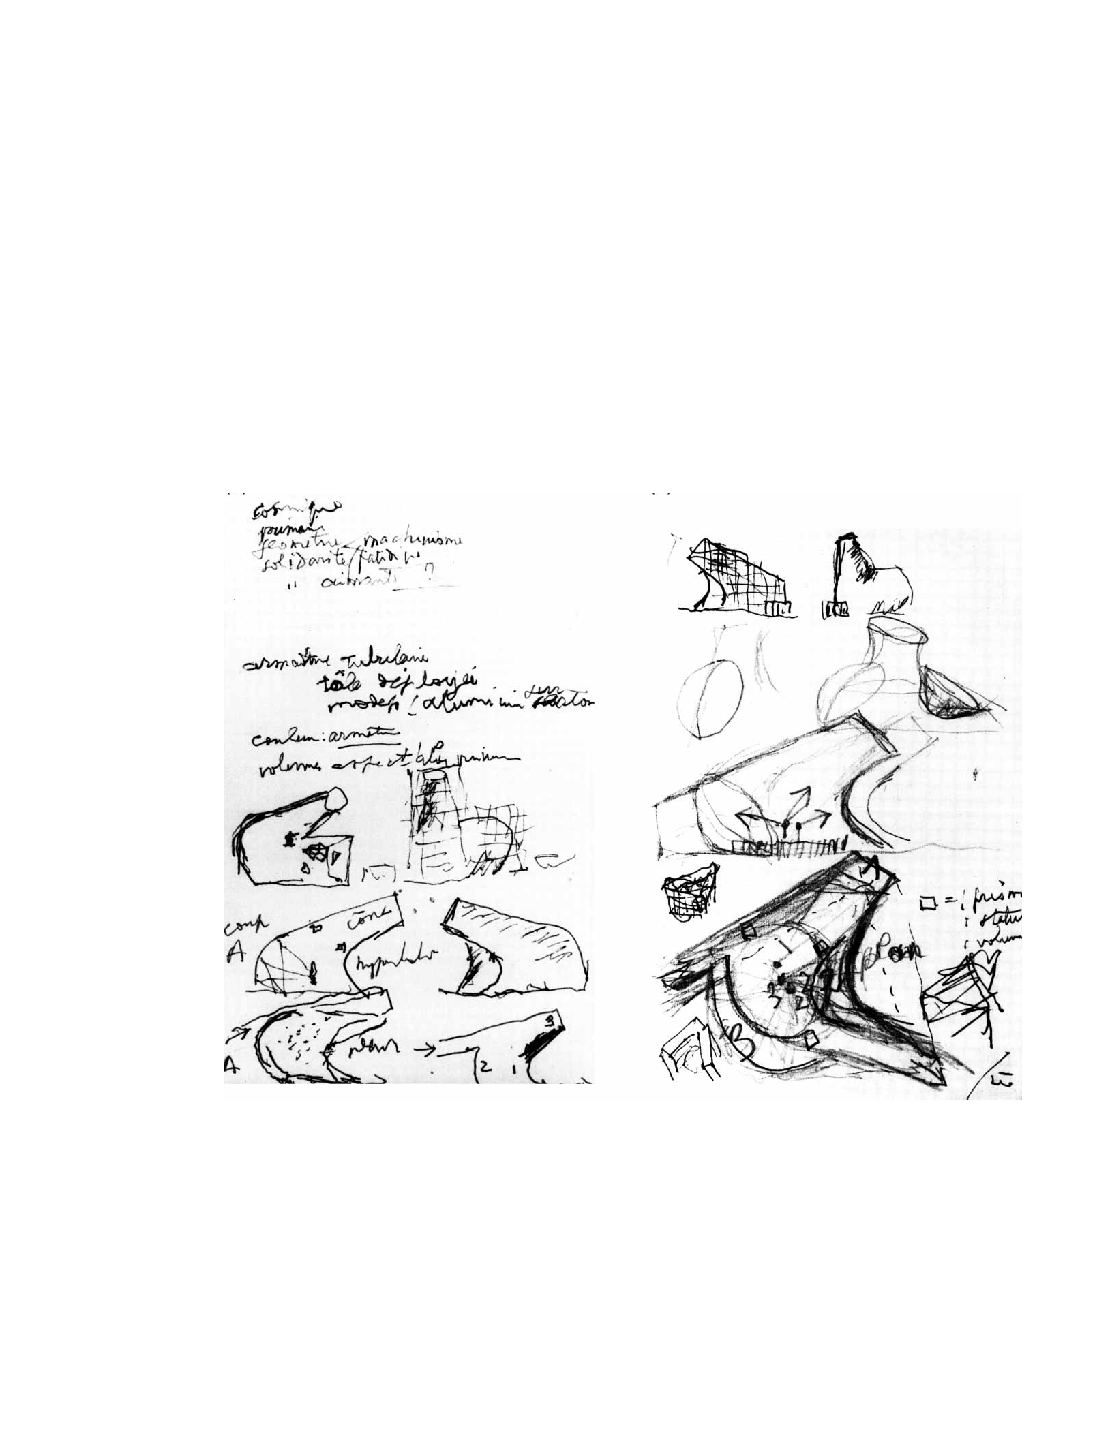
\includegraphics[width=\linewidth]{LeCorbusierDraw.pdf}
  \caption{Le Corbusier's design sketches for the Philips Pavilion,
    September \textendash{} October, 1956 (\textcircled{c} 2012
    Artists Rights Society, New York/ADAGP, Paris/FLC)}
  \label{fig:le-corbusier-sketch}
\end{figure*}

\begin{figure*}[h]
  % XenakisSketch.pdf or PhilipsDrawings.jpg
  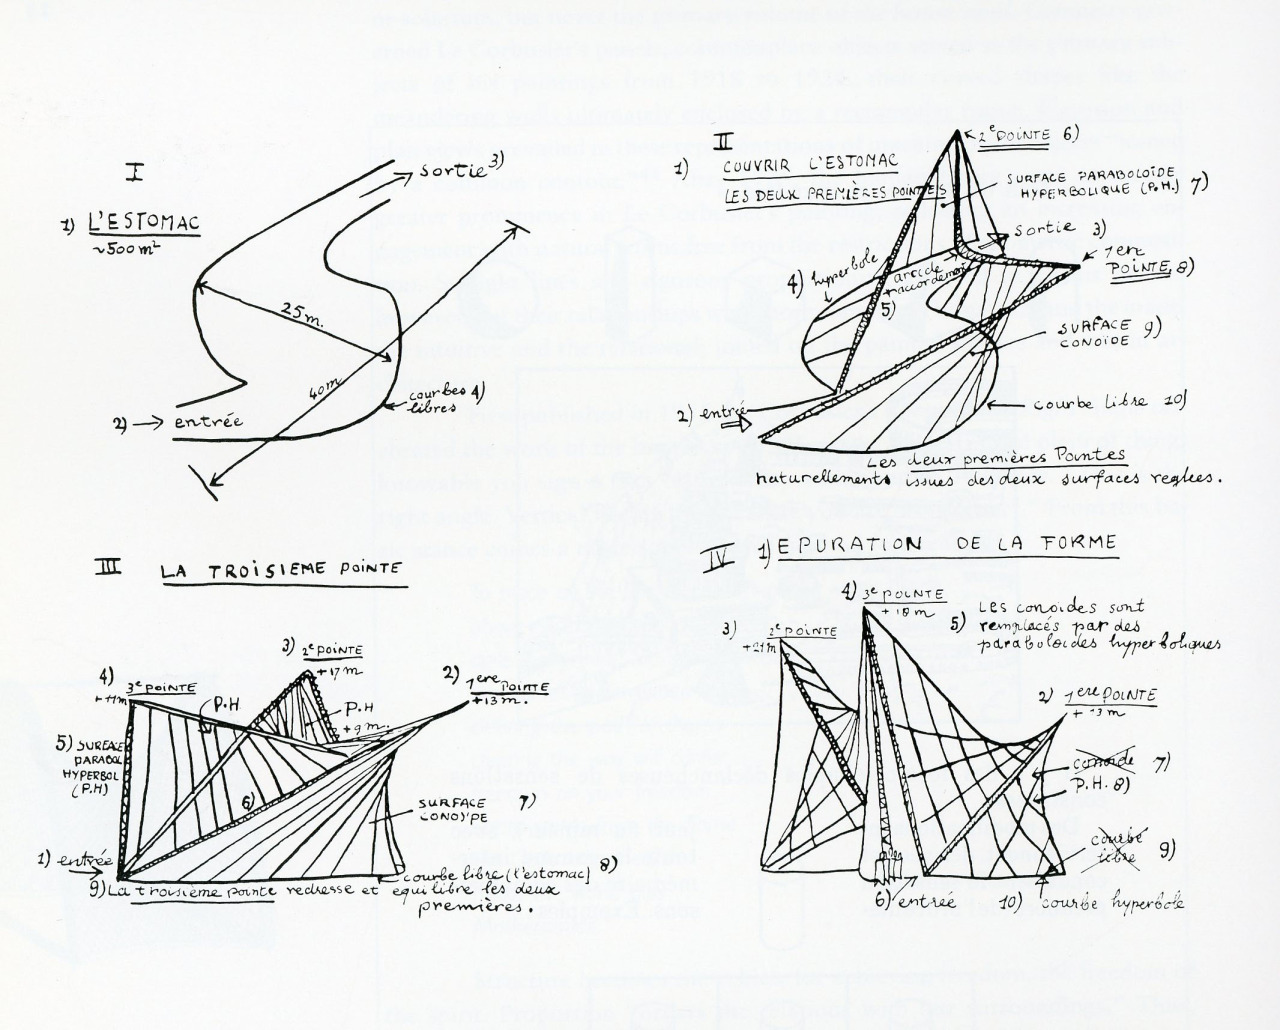
\includegraphics[]{PhilipsDrawings.jpg}
  \caption{Xenakis' early drawings of the Philips Pavilion as
    documented in volume 20 of the \textit{Philips Technical Review}.}
  \label{fig:xenakis-draw}
\end{figure*}

\section{Architecture and Music in Space and Time}
\label{sec:introduction-conclusion}

In \textit{Formalized Music},\cite{xenakis1992formalized} Xenakis
describes how developments in music theory mimic equivalent
developments in philosophy, mathematics, and the sciences. Plato, for
example, believed that all events transpire as determined by cause and
effect. While Plato and Aristotle both described causality in their
writing, it was not until the 17th century that controlled experiments
and mathematics corroborated the theory.\sidenote{In 1687, Isaac
  Newton published \textit{Philosophi\ae{} Naturalis Principia
    Mathematica} (\textit{Mathematical Principles of Natural
    Philosophy}), in which he compiled the 3 laws of motion that set
  the foundation for the study of \emph{classical mechanics}.}
Similarly, historical music follows deterministic progressions, and
music theory employs causal rules to describe counterpoint, tonality,
and harmonic movement.

Causality was largely used to describe physical phenomena until the
19th century when statistical theories in physics began to include
probabilistic notions.\sidenote{The Maxwell-Boltzmann distribution,
  which was first derived by James Clerk Maxwell in 1860, describes
  the probability distribution for the speed of a particle within an
  idealized gas. For more see
  \url{http://plato.stanford.edu/entries/statphys-statmech/}} Xenakis
noticed that more contemporary fields like \emph{probability theory}
and \emph{fuzzy logic} generalize and expand on the antecedent
theories of causality.

Xenakis thought that music composition should naturally follow
the progression that physics did, with the theory of music
generalizing and expanding on causal rules that had existed
previously. Indeed, starting in the late 19th century, and early 20th
century, composers like Strauss and Debussy began to bend the existing
rules of music theory, composing music that branched away from the
causal and tonal theories of the time. With the rise of
serialism\sidenote{Serialism is a technique for musical composition in
  which instances of musical elements (such as pitch, dynamics, or
  rhythm), are given numerical values. Sequences built from the values
  are ordered, repeated and manipulated throughout the composition.}
and indeterminate music\sidenote{In music, indeterminacy refers to the
  use of chance (such as rolling dice, or flipping coins) as part of
  the compositional process.}, composers such as Strauss, Debussy,
Stockhausen, Boulez, John Cage, Aaron Copland, and B\'{e}la Bart\'{o}k
began to use probability and chance in composition, the same way that
physicists were using probability to describe the material
world. However, to Xenakis' mathematical mind, serial music was no
less causal than the music it intended to supersede. He described
serial music as embodying ``virtually absolute
determinism.''\cite{xenakis1992formalized} Xenakis saw music theory as
a sub-set of mathematics and algebra. While musicians have a different
vocabulary, they also use mathematical principles to describe and
compose music. Because he understood mathematics as well as music, he
was able to identify how even in serialism and indeterminate music,
composers were only utilizing a small subset of algebraic theory. In
his own music, Xenakis wanted to generalize and expand the causal
framework that musicians and theorists had been using to compose and
understand music. This paralleled the developments in physics and
mathematics that helped him to form his opinions about music theory.
As a reference to \emph{chance} or \emph{stochos} Xenakis coined the
term \emph{stochastic music} to describe his development.

In \textit{Formalized Music}, Xenakis formally explains stochastic
music. It should be noted that some authors have interpreted his
description more explicitly. In \textit{Audible Design}, Trevor
Wishart, describes the stochastic process used to compose stochastic
music as:
\begin{quotation}
  ``A process in which the probabilities of proceeding from one state,
  or set of states. to another, is defined. The temporal evolution of
  the process is therefore governed by a kind of weighted
  randomness. which can be chosen to give anything from an entirely
  determined outcome, to an entirely unpredictable
  one.''\cite{Wishart1994}
\end{quotation}
It could be that the lack of a single clear definition by Xenakis is
the reason that few composers today identify as writing stochastic
music.

\paragraph{Xenakis' Reflection} In the Spring of 1976, Xenakis was
defending his doctoral thesis at the University of Paris. A
translation of his defense includes this statement:
\begin{quotation}
  ``The artist-conceptor will have to be knowledgeable and inventive
  in such varied domains as mathematics, logic, physics, chemistry,
  biology, genetics, paleontology (for the evolution of forms), the
  human sciences, and history; in short, a sort of
  \emph{universality}, but one based upon, guided by and oriented
  toward forms and architectures.'' \cite{russolo1986art}
\end{quotation}
From Xenakis' drawings we can deduce that he used the same tools,
skills, and philosophy to imagine and conceive both music and
space. His approach elevated both forms, and blurred the distinction
between the two. Maybe if we had kept using pen and paper to design
buildings and write music, the reality today would be closer to the
ideal that he imagined. Today, software for creating architecture or
composing music still favor corners to curves, and static pitches to
glissandi. More importantly, the software skills that we use to design
and manipulate space, and the skills that we use to compose music
mutually exclude each other.

This is where the projects described here make a contribution. As the
ideas that inspired Xenakis and other progressive 20th century
composers were taking root in contemporary music, the culture of
artistic form and composition was already beginning the transition
into the digital domain. However, there is no reason why digital tools
cannot favor stochastic procesees to linearity. There is no reason why
digital tools cannot treat music and architecture as equals. By
drawing from music, mathematics, computer science, acoustics, audio
engineering and mixing, sound reinforcement, multimedia production,
and live performance, we can create tools that allow us to
indiscriminately compose with space and sound.

\section{Universality}
\label{sec:universality}
At the MIT Media Lab, we celebrate the study and practice of projects
that exist outside of established academic disciplines. The Media Lab
(and the media) have described this approach as interdisciplinary,
cross-disciplinary, anti-disciplinary, or post-disciplinary;
emphasizing the clich\'{e} that traditional academics must become
experts in their field, and while narrowing their focus, they learn
\textit{more and more about less and less}, and eventually know
\textit{everything about nothing}.  \thesis is truly a Media Lab
project. It documents the creative process throughout the design,
development, and performance of a new type of audio signal
processor. In doing so, it draws from music, mathematics, computer
science, acoustics, audio engineering and mixing, sound reinforcement,
multimedia production, and live performance. How can we describe and
document a project with such broad subject material? Within a single
discipline, there is an accepted hierarchy of concepts, and we are
expected to develop a \emph{deep} understanding that penetrates this
hierarchy. We expect students to be literate in algebra, geometry and
calculus before studying physics. When we describe a physics problem,
we depend on an established collection of language, notation, and
theory.

This example reveals the curious tension between breadth and depth:
The \textit{depth} of a disciplinary approach provides the language
and abstraction that enable us to describe content and communicate at
a high level. Depth is essential for solving non-trivial
problems. However, solutions to the most complex and interesting
real-world projects always span multiple disciplines. It appears we
need breadth \emph{and} depth simultaneously.

One of the goals of this thesis is to bridge disciplines by describing
the material in a way that is accessible to readers that are not
experts in the all the fields involved. The success of the Philips
Pavilion suggests the inherent value of the 


The challenge is to describe interdisciplinary projects so that it is
accessible to readers from all disciplines. This thesis proposes the
motivation for documenting media that exists outside of established
disciplines. It proposes a strategy for such documentation, and
employs this strategy by documenting the theory, implementation, and
application of \thesis.



%%% Local Variables:
%%% mode: latex
%%% TeX-master: "CharlesHolbrow_MAS_Thesis"
%%% End:
